\section{Ход работы}
\subsection{Измерения}
1. Для начала измерены или записаны некоторые величины:
\begin{center}
    длина рычага $l = 120 \pm 1$ мм,

    частота вращения ротора (будем брать ее за эталон) $\nu = 390$ Гц,

    период обращения гироскопа $T = 3,1$ с,

    период обращения цилиндра $T_{\text{ц}} = 4,1$ с,

    масса цилиндра $M_\text{ц} = 1616,7$ г,

    диаметр цилиндра $D = 78$ мм.
\end{center}

2. Далее для разных масс измерены угол отклонения по вертикали (в гардусах) и
период:
\begin{center}
\begin{tabular}{|c|c|c|c|c|}
    \hline
    Вес, г& Период (1), с& $\Delta\varphi$ (1)& Период (2), с& $\Delta\varphi$ (2)\\
    \hline
    57 & 180.0 & 15.0 & 180.0 & 11.0\\
    \hline
    77 & 129.0 & 10.0 & 133.0 & 5.7\\
    \hline
    93 & 108.0 & 10.0 & 109.0 & 7.0\\
    \hline
    116 & 88.0 & 6.3 & 87.0 & 2.5\\
    \hline
    141 & 71.0 & 5.0 & 71.5 & 7.3\\
    \hline
    176 & 57.0 & 3.0 & 57.5 & 6.3\\
    \hline
    220 & 45.5 & 4.8 & 46.3 & 10.0\\
    \hline
    273 & 37.0 & 5.7 & 37.0 & 5.7\\
    \hline
    343 & 29.5 & 5.0 & 29.7 & 6.6\\
    \hline
\end{tabular}
\end{center}
\subsection{Обработка}

3. Для начала посчитаем момент инерции гироскопа по формуле (номер):
\begin{equation*}
    I = I_\text{ц}\cdot\frac{T^2}{T_\text{ц}^2} = \frac{M_\text{ц}D^2T^2}{8T_\text{ц}^2} \approx 5 \cdot 10^{-4} \text{ кг}\cdot\text{м}^2.
\end{equation*}

4. Теперь построим график зависимости
$m\left(\frac 1T\right) = m\left(\nu\right)$:
\begin{figure}[H]
    \centering
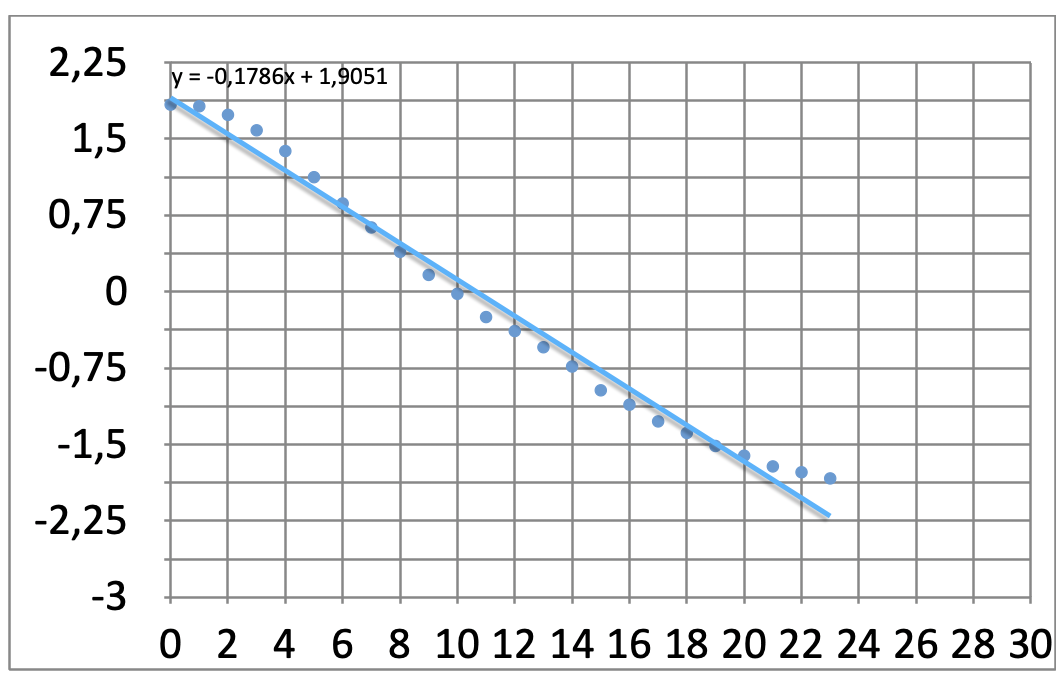
\includegraphics[width=0.7\linewidth,center]{p4.png}
    \label{fig:my_label}
\end{figure}
Угол наклона прямой $k = (985 \pm 2) \cdot 10^{-4}\text{ }\frac{\text{г}}{\text{кГц}}$.

5. Из формулы (8) получаем выражение для угловой частоты вращения
ротора:
\begin{equation*}
    \omega_0 = \frac{kgl}{2\pi I_z} \approx 369.1 \pm 0.4 \text{ Гц}.
\end{equation*}

6. Построим график для угловой скорости, изменяющей наклон
гироскопа:

\begin{figure}[H]
    \centering
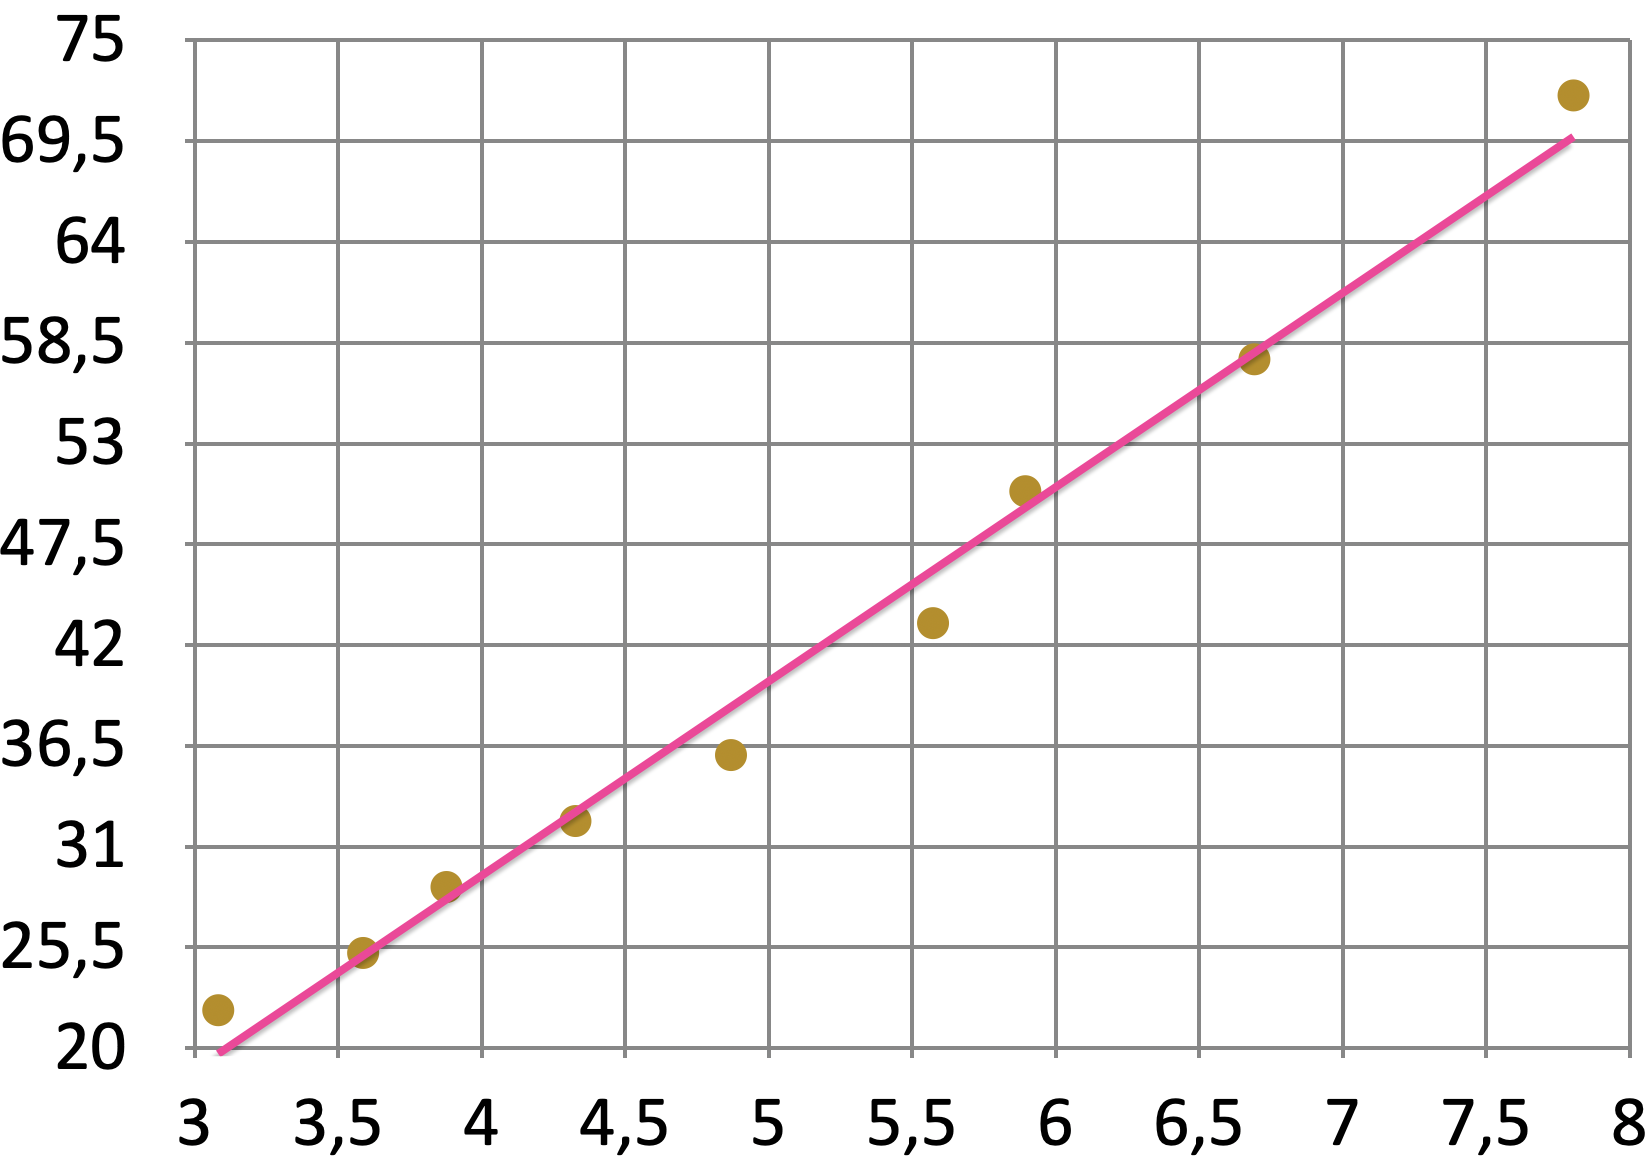
\includegraphics[width=\linewidth,center]{p5.png}
    \label{fig:my_label}
\end{figure}
Угол наклона в каждом из случаев $0,0003$ и $0,0007$ соответственно,
что бренебрежительно мало, поэтому можно считать, что угловая
скорость неизменна.

7. Получим значение для угловой скорости:
\begin{equation*}
    \Omega_\text{тр} = \left(1,92 \pm 0,05\right)  \frac{^\circ}{\text{с}}.
\end{equation*}

8. Посчитаем момент силы трения:
\begin{equation*}
    M_\text{тр} = L\Omega_\text{тр} = I\omega_0\Omega_\text{тр} = \left(62 \pm 2\right) \text{ мН} \cdot \text{м}.
\end{equation*}
